\chapter{Taking Advantage of the Internet}







The Internet provides a wealth of data spanning the world, access
to sophisticated statistical computing, and a practical means for
you to communicate with your own students.  In this chapter, we'll
illustrate some mundane ways for you to distribute and share data and
software with your students, web-based interfaces for statistical
computing,  as well as tools for ``scraping'' data
from the Internet using application program interfaces (API's) or
through XML (eXtensible Markup Language).   

We draw your attention particularly to 
provocative papers by Gould \cite{Goul:2010} and Nolan and Temple Lang
\cite{nola:temp:2010}, who
highlight the importance of broadening the type of data students encounter
in their first courses as well as the role of computing in modern statistics, respectively.
\FoodForThought{The wealth of data accessible to students on the internet
continues to increase at what feels like an exponential rate.}

\section{Sharing With and Among Your Students}
\label{sec:distributing-data}

Instructors often have their own data sets to illustrate 
points of statistical interest or to make a particular connection with
a class.  Sometimes you may want your class as a whole to construct a
data set, perhaps by filling in a survey or by contributing
their own small bit of data to a class collection.  Students may be
working on projects in small groups; it's nice to have tools to
support such work so that all members of the group have access to the
data and can contribute to a written report.

There are now many technologies for supporting such sharing.  For the
sake of simplicity, we will emphasize three that we have found
particularly useful both in teaching statistics and in our
professional collaborative work.  These are:
\begin{itemize}
\item A web site with minimal overhead, such as provided by Dropbox.
\item The services of Google Docs.
\item A web-based \RStudio\ server for \R.
\end{itemize}
The first two are already widely used in university environments and
are readily accessible simply by setting up accounts.  Setting up an
\RStudio\ web server requires some IT support, but is well within the
range of skills found in IT offices and even among some individual faculty.

\subsection{Your Own Web Site}

You may already have a web site.  We have in mind a place where you
can place files and have them accessed directly from the Internet.
For sharing data, it's best if this site is public, that is, it does not require a login.
That rules out most ``course support'' systems such as Moodle or
Blackboard.  
\FoodForThought{Our discussion of Dropbox is primarily for those who do
not already know how to do this other ways.}%

The Dropbox service for storing files in the ``cloud'' provides a very
convenient way to distribute files over the web.  (Go to
\texttt{dropbox.com} for information and to sign up for a free account.)
Dropbox is routinely used to provide automated backup and coordinated
file access on multiple computers.  But the Dropbox service also
provides a {\sc Public} directory.  Any files that you place in that
directory can be accessed directly by a URL.  

To illustrate, suppose you wish to share some data set with your
students.  You've constructed this data set in a spreadsheet and
stored it as a CSV file, let's call it ``example-A.csv''.  Move this
file into the {\sc Public} directory under Dropbox --- on most
computers Dropbox arranges things so that its directories appear
exactly like ordinary directories and you'll use the ordinary familiar
file management techniques as in Figure \ref{fig:dropbox1}.
\begin{figure}
\begin{center}
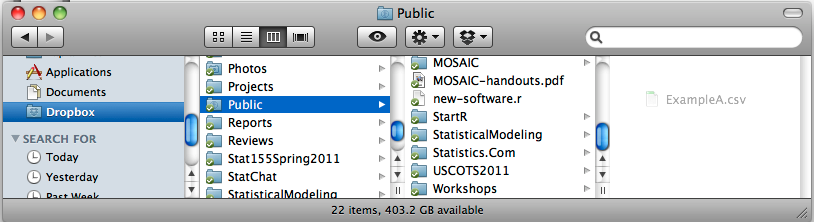
\includegraphics[width=3.5in]{images/dropbox1.png}
\end{center}
\caption{\label{fig:dropbox1} Dragging a CSV file to a Dropbox Public directory}
\end{figure}

Dropbox also makes it straightforward to construct the web-location
identifying URL for any file by using mouse-based menu commands to
place the URL into the clipboard, whence it can be copied to your
course-support software system or any other place for distribution to
students.  For a CSV file, reading the contents of the file into \R\
can be done with the \function{read.csv} function, by giving it the
quoted URL:
\begin{knitrout}
\definecolor{shadecolor}{rgb}{.97, .97, .97}{\color{fgcolor}\begin{kframe}
\begin{flushleft}
\ttfamily\noindent
\hlsymbol{a}{\ }\hlassignement{\usebox{\hlnormalsizeboxlessthan}-}{\ }\hlfunctioncall{read.csv}\hlkeyword{(}\hlstring{"{}http://dl.dropbox.com/u/5098197/USCOTS2011/ExampleA.csv"{}}\hlkeyword{)}\mbox{}
\normalfont
\end{flushleft}
\end{kframe}}
\end{knitrout}

\InstructorNote{The history feature in \RStudio\ can be used to 
re-run this command in future sessions}

\begin{figure}
\begin{center}
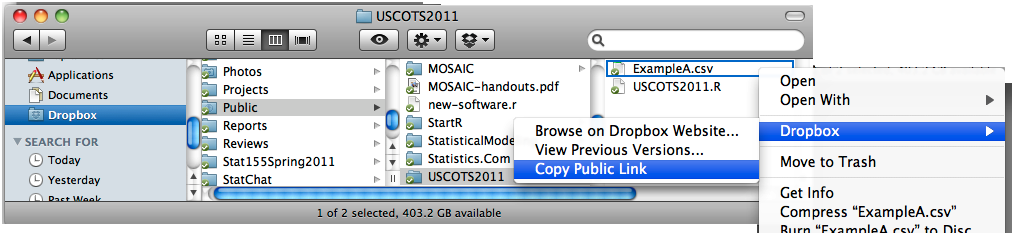
\includegraphics[width=4.5in]{images/dropbox2.png}
\end{center}
\caption{\label{fig:dropbox2}Getting the URL of a file in a Dropbox Public directory}
\end{figure}

This technique makes it easy to distribute data with little
advance preparation.  It's fast enough to do in the middle of a
class: the CSV file is available to your students (after a brief lag
while Dropbox synchronizes).  
It can even be edited by you (but not by your students).

The same technique can be applied to all sorts of files: for example,
\R\ workspaces or even \R\ scripts.  Of course, your students need to
use the appropriate \R\ command: \function{load()} for a workspace or
\function{source()} for a script.

It's a good idea to create a file with your course-specific \R\
scripts, adding on to it and modifying it as the course progresses.
This allows you to distribute all sorts of special-purpose functions,
letting you distribute new \R\ material to your students.  For
instance, that brilliant new ``manipulate'' idea you had at 2am can be
programmed up and put in place for your students to use the next
morning in class.  Then as you identify bugs and refine the program,
you can make the updated software immediately available to your students.

For example, in the next section of this book we will discuss reading
directly from Google Spreadsheets.  It happens that we wanted to try a
new technique but were not sure that it was worth including in the
\texttt{mosaic} package.  So, we need another way to distribute it to
you.  Use this statement:
\begin{knitrout}
\definecolor{shadecolor}{rgb}{.97, .97, .97}{\color{fgcolor}\begin{kframe}
\begin{flushleft}
\ttfamily\noindent
\hlfunctioncall{source}\hlkeyword{(}\hlstring{"{}http://dl.dropbox.com/u/5098197/USCOTS2011/USCOTS2011.R"{}}\hlkeyword{)}\mbox{}
\normalfont
\end{flushleft}
\end{kframe}}
\end{knitrout}

Among other things, the operator \texttt{readGoogleCSV()} is defined
in the script that gets sourced in by that command.  Again, you can
edit the file directly on your computer and have the results instantly
available (subject only to the several second latency of Dropbox) to
your students.  Of course, they will have to re-issue the
\function{source} command to re-read the script.

If privacy is a concern, for instance if you want the data available
only to your students, you can effectively accomplish this 
by giving files names known only to your students, e.g.,
``Example-A78r423.csv''.  

\Caution{\emph{Security through Obscurity} of this sort will 
not generally satisfy institutional data protection regulations}



\subsection{GoogleDocs}

The Dropbox technique is excellent for broadcasting: taking files you
create and distributing them in a read-only fashion to your students.
But when you want two-way or multi-way
sharing of files, other techniques are called for, such as provided by
the GoogleDocs service.

GoogleDocs allows students and instructors to create various forms of
documents, including reports, presentations, and spreadsheets. (In
addition to creating documents {\em de novo}, Google will also convert
existing documents in a variety of formats.)

Once on the GoogleDocs system, the documents can be edited 
{\em  simultaneously} by multiple users in different locations.  They
can be shared with individuals or groups and published for
unrestricted viewing and even editing.

For teaching, this has a variety of uses:
\begin{itemize}
  \item Students working on group projects can all simultaneously have
    access to the report as it is being written and to data that is
    being assembled by the group.
  \item The entire class can be given access to a data set, both for
    reading and for writing.
  \item The Google Forms system can be used to construct surveys, the
    responses to which automatically populate a spreadsheet that can
    be read by the survey creators.
  \item Students can ``hand in'' reports and data sets by copying a link
    into a course support system such as Moodle or Blackboard, or
    emailing the link.
  \item The instructor can insert comments and/or corrections directly
    into the document.
\end{itemize}

An effective technique for organizing student work and ensuring
that the instructor (and other graders) have access to it, is to
create a separate Google directory for each student in your class
(Dropbox can also be used in this manner).
Set the permission on this directory to share it with the
student.  Anything she or he drops into the directory is automatically
available to the instructor.  The student can also share with specific
other students (e.g., members of a project group).

\begin{example}
One exercise for students starting out in a statistics course is to
collect data to find out whether the ``close door'' button on an
elevator has any effect.  This is an opportunity to introduce simple
ideas of experimental design.  But it's also a chance to teach about
the organization of data.

Have your students, as individuals or small groups, study a particular
elevator, organize their data into a spreadsheet, and hand in their
individual spreadsheet.  Then review the spreadsheets in class.  You
will likely find that many groups did not understand clearly the
distinction between cases and variables, or coded their data in
ambiguous or inconsistent ways.

Work with the class to establish a consistent scheme for the variables
and their coding, e.g.,  a variable \VN{ButtonPress} with levels
``Yes'' and ``No'',  a variable \VN{Time} with the time in seconds
from a fiducial time (e.g. when the button was pressed or would have
been pressed) with time measured in seconds, and variables \VN{ElevatorLocation}
and \VN{GroupName}.  Create a spreadsheet
with these variables and a few cases filled in.  Share it with the class.

Have each of your students add his or her own data to the class data
set.  Although this is a trivial task, having to translate their
individual data into a common format strongly reinforces the
importance of a consistent measurement and coding system for recording
data. 
\end{example}

Once you have a spreadsheet file in GoogleDocs, you will want to open
it in \R.  Of course, it's possible to export it as a CSV file, then
open it using the CSV tools in \R, such as \function{read.csv}.
But there are easier ways that let you work with the data ``live.''

\paragraph{In the web-server version of \RStudio,} described below, you can
  use a menu item to locate and load your spreadsheet.

\begin{center}
  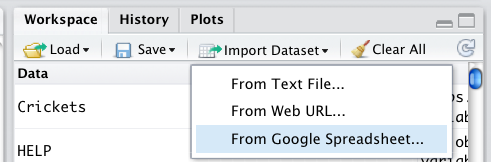
\includegraphics[width=3in]{images/google-spreadsheet1.png}
\end{center}

\paragraph{If you are using other \R\ interfaces,} you must first use the Google
  facilities for publishing documents.
\begin{enumerate}
  \item From within the document, use the ``Share'' dropdown menu and
    choose ``Publish as a Web Page.''
   \item Press the ``Start Publishing'' button in the ``Publish to the
     web'' dialog box. (See figure \ref{fig:publish-google}.)
   \item In that dialog box, go to ``Get a link to the published
     data.''  Choose the CSV format and copy out the link that's
     provided.  You can then publish that link on your web site, or via
     course-support software.  Only people with the link can see the
     document, so it remains effectively private to outsiders.
\end{enumerate}


\begin{figure}
\begin{center}
  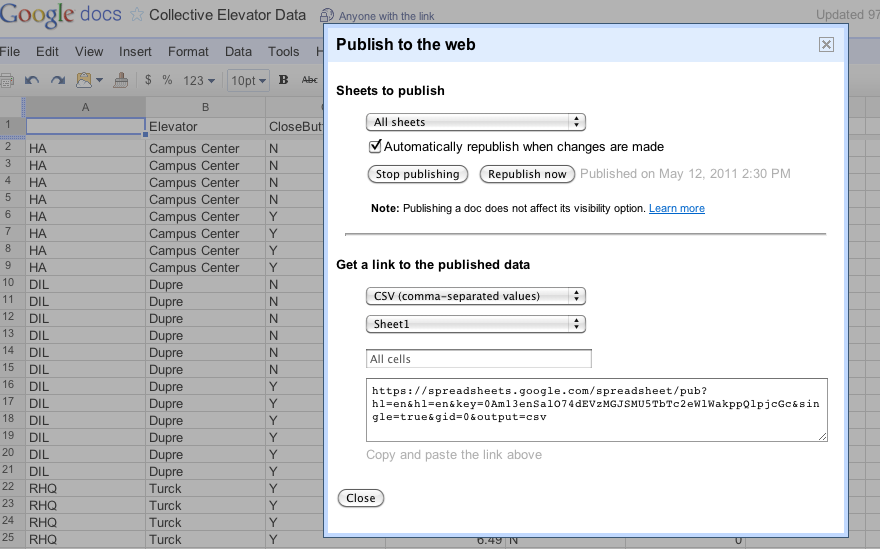
\includegraphics[width=4.5in]{images/publishing-google1.png}
\end{center}
\caption{\label{fig:publish-google}Publishing a Google Spreadsheet so that it can be read
    directly into \R.}
\end{figure}

It turns out that communicating with GoogleDocs requires facilities
that are not present in the base version of \R, but are available
through the \texttt{RCurl} package.  In order to make these readily
available to students, we have created a function that takes a quoted
string with the Google-published URL and reads the corresponding file
into a data frame:
\begin{knitrout}
\definecolor{shadecolor}{rgb}{.97, .97, .97}{\color{fgcolor}\begin{kframe}
\begin{flushleft}
\ttfamily\noindent
\hlsymbol{elev}{\ }\hlassignement{\usebox{\hlnormalsizeboxlessthan}-}{\ }\hlfunctioncall{readGoogleCSV}\hlkeyword{(}\hlstring{"{}https://spreadsheets.google.com/spreadsheet/pub?hl=en\usebox{\hlnormalsizeboxand}hl=en\usebox{\hlnormalsizeboxand}key=0Am13enSalO74dEVzMGJSMU5TbTc2eWlWakppQlpjcGc\usebox{\hlnormalsizeboxand}single=TRUE\usebox{\hlnormalsizeboxand}gid=0\usebox{\hlnormalsizeboxand}output=csv"{}}\hlkeyword{)}\mbox{}
\normalfont
\end{flushleft}
\begin{verbatim}
Loading required package: RCurl
\end{verbatim}
\begin{verbatim}
Loading required package: bitops
\end{verbatim}
\begin{flushleft}
\ttfamily\noindent
\hlfunctioncall{head}\hlkeyword{(}\hlsymbol{elev}\hlkeyword{)}\mbox{}
\normalfont
\end{flushleft}
\begin{verbatim}
  StudentGroup      Elevator CloseButton  Time Enroute LagToPress
1           HA Campus Center           N 8.230       N          0
2           HA Campus Center           N 7.571       N          0
3           HA Campus Center           N 7.798       N          0
4           HA Campus Center           N 8.303       N          0
5           HA Campus Center           Y 5.811       N          0
6           HA Campus Center           Y 6.601       N          0
\end{verbatim}
\end{kframe}}
\end{knitrout}


Of course, you'd never want your students to type that URL by hand;
you should provide it in a copy-able form on a web site or within a
course support system.

Note that the \function{readGoogleCSV} function is not part of the
\texttt{mosaic} package.  As described previously, we make it
available via an \R\ source file that can be read into the current
session of \R\ using the \function{source} command:
\begin{knitrout}
\definecolor{shadecolor}{rgb}{.97, .97, .97}{\color{fgcolor}\begin{kframe}
\begin{flushleft}
\ttfamily\noindent
\hlfunctioncall{source}\hlkeyword{(}\hlstring{"{}http://dl.dropbox.com/u/5098197/USCOTS2011/USCOTS2011.R"{}}\hlkeyword{)}\mbox{}
\normalfont
\end{flushleft}
\end{kframe}}
\end{knitrout}





\subsection{The \RStudio\ Web Server}

\RStudio\ is available as a desktop application that provides a
considerately designed interface to the standard \R\ software that you
can install on individual computers.

But there is another version of \RStudio\ available, one that takes
the form of a web server.  There are some substantial advantages to
using the web-server version.
\begin{itemize}
\item For the user, no installation is required beyond a standard web browser.
\item Sessions are continued indefinitely; you can come back to your
  work exactly where you left it.
\item A session started on one computer can be continued on another
  computer.  So a student can move seamlessly from the classroom to
  the dorm to a friend's computer.  
\item The web-server system provides facilities for direct access to
  GoogleDocs.
\end{itemize}


As \RStudio\ continues to be developed, we anticipate facilities being
added that will enhance even more the ability to teach with R:

\Caution{These are anticipated future features.}


\begin{itemize}
\item
The ability to create URLs that launch \RStudio\ and read in a data set all in a single 
click.
\item The ability to share sessions simultaneously, so that more than
  one person can be giving commands.  This will be much like Google Docs, but with the
  \R\ console as the document.   Imagine being able to start a
  session, then turn it over to a student in your classroom to give
  the commands, with you being able to make corrections as needed.
\item The ability to clone sessions and send them off to others.  For
  instance, you could set up a problem then pass it along to your
  students for them to work on.  
\end{itemize}

But even with the present system, the web-based \RStudio\ version
allows you to work with students effectively during office hours.  You
can keep your own version of \RStudio\ running in your usual browser, but give your visiting a
student a window in a new browser: Firefox, Chrome, Safari, Internet
Explorer, etc.  Each new browser is effectively a new machine, so your
student can log in securely to his or her own account.



\section{Data Mining Activities}

\begin{comment}
We end this chapter with several examples that do data mining via the Internet.
Some of these are mere glimpses into what might be possible as tools for 
accessing this kind of data become more prevalent and easier to use.
\end{comment}
\subsection{What percentage of Earth is Covered with Water?}
\label{sec:googleMap}
We can estimate the proportion of the world covered with water by randomly 
sampling points on the globe and inspecting them using GoogleMaps.

First, let's do a sample size computation.  Suppose we want to 
estimate (at the 95\% confidence level) this proportion within $\pm 5$\%.
There are several ways to estimate the necessary sample size, including
algebraically solving
\[
(1.96) \sqrt{ \hat p (1-\hat p) /n} = 0.05
\]
for $n$ given some estimated value of $\hat p$.  The \function{uniroot()} function
can solve this sort of thing numerically.  Here we take an approach 
that looks at a table of values of $n$ and $\hat p$ and margin of error.
\begin{knitrout}
\definecolor{shadecolor}{rgb}{.97, .97, .97}{\color{fgcolor}\begin{kframe}
\begin{flushleft}
\ttfamily\noindent
\hlsymbol{n}{\ }\hlassignement{\usebox{\hlnormalsizeboxlessthan}-}{\ }\hlfunctioncall{seq}\hlkeyword{(}\hlnumber{50}\hlkeyword{,}{\ }\hlnumber{500}\hlkeyword{,}{\ }\hlargument{by}{\ }\hlargument{=}{\ }\hlnumber{50}\hlkeyword{)}\hspace*{\fill}\\
\hlstd{}\hlsymbol{p.hat}{\ }\hlassignement{\usebox{\hlnormalsizeboxlessthan}-}{\ }\hlfunctioncall{seq}\hlkeyword{(}\hlnumber{0.5}\hlkeyword{,}{\ }\hlnumber{0.9}\hlkeyword{,}{\ }\hlargument{by}{\ }\hlargument{=}{\ }\hlnumber{0.1}\hlkeyword{)}\hspace*{\fill}\\
\hlstd{}\hlsymbol{margin\usebox{\hlnormalsizeboxunderscore}of\usebox{\hlnormalsizeboxunderscore}error}{\ }\hlassignement{\usebox{\hlnormalsizeboxlessthan}-}{\ }\hlkeyword{function}\hlkeyword{(}\hlformalargs{n}\hlkeyword{,}{\ }\hlformalargs{p}\hlkeyword{,}{\ }\hlformalargs{conf.level}{\ }\hleqformalargs{=}{\ }\hlnumber{0.95}\hlkeyword{)}{\ }\hlkeyword{\usebox{\hlnormalsizeboxopenbrace}}\hspace*{\fill}\\
\hlstd{}{\ }{\ }{\ }{\ }\hlkeyword{-}\hlfunctioncall{qnorm}\hlkeyword{(}\hlkeyword{(}\hlnumber{1}{\ }\hlkeyword{-}{\ }\hlsymbol{conf.level}\hlkeyword{)}\hlkeyword{/}\hlnumber{2}\hlkeyword{)}{\ }\hlkeyword{*}{\ }\hlfunctioncall{sqrt}\hlkeyword{(}\hlsymbol{p}{\ }\hlkeyword{*}{\ }\hlkeyword{(}\hlnumber{1}{\ }\hlkeyword{-}{\ }\hlsymbol{p}\hlkeyword{)}\hlkeyword{/}\hlsymbol{n}\hlkeyword{)}\hspace*{\fill}\\
\hlstd{}\hlkeyword{\usebox{\hlnormalsizeboxclosebrace}}\hspace*{\fill}\\
\hlstd{}\hlcomment{\usebox{\hlnormalsizeboxhash}{\ }calculate{\ }margin{\ }of{\ }error{\ }for{\ }all{\ }combos{\ }of{\ }n{\ }and{\ }p.hat}\hspace*{\fill}\\
\hlstd{}\hlsymbol{tbl}{\ }\hlassignement{\usebox{\hlnormalsizeboxlessthan}-}{\ }\hlfunctioncall{outer}\hlkeyword{(}\hlsymbol{n}\hlkeyword{,}{\ }\hlsymbol{p.hat}\hlkeyword{,}{\ }\hlsymbol{margin\usebox{\hlnormalsizeboxunderscore}of\usebox{\hlnormalsizeboxunderscore}error}\hlkeyword{)}\hspace*{\fill}\\
\hlstd{}\hlfunctioncall{colnames}\hlkeyword{(}\hlsymbol{tbl}\hlkeyword{)}{\ }\hlassignement{\usebox{\hlnormalsizeboxlessthan}-}{\ }\hlsymbol{p.hat}\hspace*{\fill}\\
\hlstd{}\hlfunctioncall{rownames}\hlkeyword{(}\hlsymbol{tbl}\hlkeyword{)}{\ }\hlassignement{\usebox{\hlnormalsizeboxlessthan}-}{\ }\hlsymbol{n}\hspace*{\fill}\\
\hlstd{}\hlsymbol{tbl}\mbox{}
\normalfont
\end{flushleft}
\begin{verbatim}
        0.5     0.6     0.7     0.8     0.9
50  0.13859 0.13579 0.12702 0.11087 0.08315
100 0.09800 0.09602 0.08982 0.07840 0.05880
150 0.08002 0.07840 0.07334 0.06401 0.04801
200 0.06930 0.06790 0.06351 0.05544 0.04158
250 0.06198 0.06073 0.05681 0.04958 0.03719
300 0.05658 0.05544 0.05186 0.04526 0.03395
350 0.05238 0.05132 0.04801 0.04191 0.03143
400 0.04900 0.04801 0.04491 0.03920 0.02940
450 0.04620 0.04526 0.04234 0.03696 0.02772
500 0.04383 0.04294 0.04017 0.03506 0.02630
\end{verbatim}
\end{kframe}}
\end{knitrout}

From this it appears that a sample size of approximately 300--400 will get
us the accuracy we desire.  A class of students can easily generate
this much data in a matter of minutes if each student inspects 10--20 maps.
The example below assumes a sample size of 10 locations per student.
This can be adjusted depending on the number of students and the desired
margin of error.

\begin{enumerate}
\item Generate 10 random locations.

\begin{knitrout}
\definecolor{shadecolor}{rgb}{.97, .97, .97}{\color{fgcolor}\begin{kframe}
\begin{flushleft}
\ttfamily\noindent
\hlsymbol{positions}{\ }\hlassignement{\usebox{\hlnormalsizeboxlessthan}-}{\ }\hlfunctioncall{rgeo}\hlkeyword{(}\hlnumber{10}\hlkeyword{)}\hspace*{\fill}\\
\hlstd{}\hlsymbol{positions}\mbox{}
\normalfont
\end{flushleft}
\begin{verbatim}
       lat    lon
1  -37.761  53.98
2   29.448 108.57
3   54.117 169.96
4   -1.596  55.89
5  -37.155 -83.65
6  -72.433  42.49
7   12.607  47.72
8  -61.168 -85.54
9  -10.820  64.32
10 -15.273  92.25
\end{verbatim}
\end{kframe}}
\end{knitrout}


\item
Open a GoogleMap centered at each position.

\begin{knitrout}
\definecolor{shadecolor}{rgb}{.97, .97, .97}{\color{fgcolor}\begin{kframe}
\begin{flushleft}
\ttfamily\noindent
\hlfunctioncall{googleMap}\hlkeyword{(}\hlargument{pos}{\ }\hlargument{=}{\ }\hlsymbol{positions}\hlkeyword{,}{\ }\hlargument{mark}{\ }\hlargument{=}{\ }\hlnumber{TRUE}\hlkeyword{)}\mbox{}
\normalfont
\end{flushleft}
\end{kframe}}
\end{knitrout}

You may need to turn off pop-up blocking for this to work smoothly.

\item
For each map, record whether the center is located in water or on land.  The options \option{mark=TRUE}
is used to place a marker at the center of the map (this is helpful for locations that are close to 
the coast).  
\begin{center}
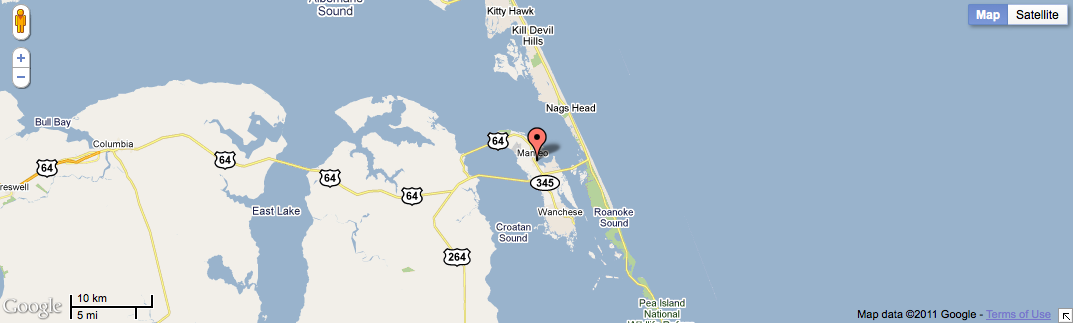
\includegraphics[width=.8\textwidth]{images/google-water1}
\end{center}
You can zoom in or out to get a better look.
\begin{center}
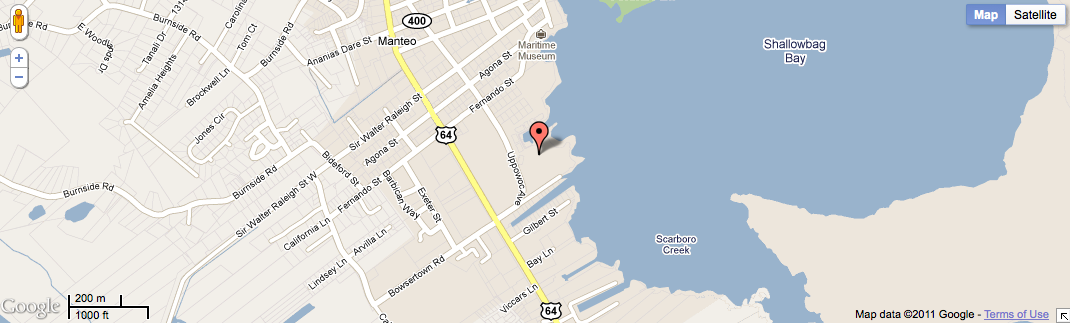
\includegraphics[width=.8\textwidth]{images/google-water2}
\end{center}


\item
Record your data in a GoogleForm at 

\begin{center}
\url{http://mosaic-web.org/uscots2011/google-water.html}
%\url{https://spreadsheets.google.com/viewform?formkey=dGREcUR6YjRLSWFTWVpNNXA5ZUZ1TXc6MQ}

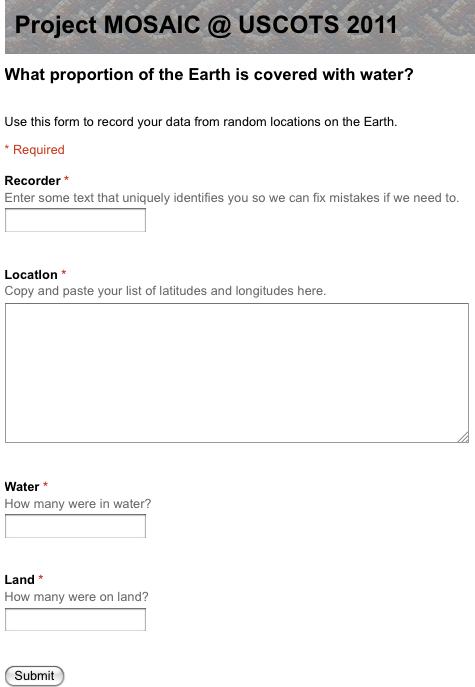
\includegraphics[width=.4\textwidth]{images/googleForm-water}
\end{center}

For the latitude and longitude information, simply copy and paste the output of 
\begin{knitrout}
\definecolor{shadecolor}{rgb}{.97, .97, .97}{\color{fgcolor}\begin{kframe}
\begin{flushleft}
\ttfamily\noindent
\hlsymbol{positions}\mbox{}
\normalfont
\end{flushleft}
\end{kframe}}
\end{knitrout}

\Caution{This sort of copy-and-paste operation works better in some 
browsers (Firefox) than in others (Safari).}%
\item
After importing the data from Google, it is simple to sum the counts across the class.




\begin{knitrout}
\definecolor{shadecolor}{rgb}{.97, .97, .97}{\color{fgcolor}\begin{kframe}
\begin{flushleft}
\ttfamily\noindent
\hlfunctioncall{sum}\hlkeyword{(}\hlsymbol{googleData}\hlkeyword{\usebox{\hlnormalsizeboxdollar}}\hlsymbol{Water}\hlkeyword{)}\mbox{}
\normalfont
\end{flushleft}
\begin{verbatim}
[1] 215
\end{verbatim}
\begin{flushleft}
\ttfamily\noindent
\hlfunctioncall{sum}\hlkeyword{(}\hlsymbol{googleData}\hlkeyword{\usebox{\hlnormalsizeboxdollar}}\hlsymbol{Land}\hlkeyword{)}\mbox{}
\normalfont
\end{flushleft}
\begin{verbatim}
[1] 85
\end{verbatim}
\end{kframe}}
\end{knitrout}


Then use your favorite method of analysis, perhaps \function{binom.test()}.

\begin{knitrout}
\definecolor{shadecolor}{rgb}{.97, .97, .97}{\color{fgcolor}\begin{kframe}
\begin{flushleft}
\ttfamily\noindent
\hlfunctioncall{interval}\hlkeyword{(}\hlfunctioncall{binom.test}\hlkeyword{(}\hlnumber{215}\hlkeyword{,}{\ }\hlnumber{300}\hlkeyword{)}\hlkeyword{)}{\ }{\ }\hlcomment{\usebox{\hlnormalsizeboxhash}{\ }numbers{\ }of{\ }successes{\ }and{\ }trials}\mbox{}
\normalfont
\end{flushleft}
\begin{verbatim}
probability of success                  lower                  upper 
                0.7167                 0.6620                 0.7670 
\end{verbatim}
\end{kframe}}
\end{knitrout}

\end{enumerate}


\subsection{Roadless America}

The \function{rgeo()} function can also sample within a latitude longitude ``rectangle".
This allows us to sample subsets of the globe.  In this activity we will estimate 
the proportion of the continental United States that is within 1 mile of a road.

\begin{enumerate}
\item
Generate a random sample of locations in a box containing the continental United States.
Some of these points may be in Canada, Mexico, an ocean or a major lake.  These 
will be discarded from our sample before making our estimate.
\begin{knitrout}
\definecolor{shadecolor}{rgb}{.97, .97, .97}{\color{fgcolor}\begin{kframe}
\begin{flushleft}
\ttfamily\noindent
\hlsymbol{positions}{\ }\hlassignement{\usebox{\hlnormalsizeboxlessthan}-}{\ }\hlfunctioncall{rgeo}\hlkeyword{(}\hlnumber{10}\hlkeyword{,}{\ }\hlargument{lonlim}{\ }\hlargument{=}{\ }\hlfunctioncall{c}\hlkeyword{(}\hlkeyword{-}\hlnumber{125}\hlkeyword{,}{\ }\hlkeyword{-}\hlnumber{65}\hlkeyword{)}\hlkeyword{,}{\ }\hlargument{latlim}{\ }\hlargument{=}{\ }\hlfunctioncall{c}\hlkeyword{(}\hlnumber{25}\hlkeyword{,}{\ }\hlnumber{50}\hlkeyword{)}\hlkeyword{)}\hspace*{\fill}\\
\hlstd{}\hlsymbol{positions}\mbox{}
\normalfont
\end{flushleft}
\begin{verbatim}
     lat     lon
1  49.86  -89.68
2  31.74  -92.11
3  28.72  -89.35
4  28.16  -76.41
5  33.85  -99.57
6  34.77  -81.19
7  46.61 -109.52
8  40.13  -90.41
9  42.50  -71.65
10 43.86 -123.74
\end{verbatim}
\end{kframe}}
\end{knitrout}


\item
Open a GoogleMap centered at each position.  This time we'll zoom in a bit and add 
a circle of radius 1 to our map.

\begin{knitrout}
\definecolor{shadecolor}{rgb}{.97, .97, .97}{\color{fgcolor}\begin{kframe}
\begin{flushleft}
\ttfamily\noindent
\hlfunctioncall{googleMap}\hlkeyword{(}\hlargument{pos}{\ }\hlargument{=}{\ }\hlsymbol{positions}\hlkeyword{,}{\ }\hlargument{mark}{\ }\hlargument{=}{\ }\hlnumber{TRUE}\hlkeyword{,}{\ }\hlargument{zoom}{\ }\hlargument{=}{\ }\hlnumber{12}\hlkeyword{,}{\ }\hlargument{radius}{\ }\hlargument{=}{\ }\hlnumber{1}\hlkeyword{)}\mbox{}
\normalfont
\end{flushleft}
\end{kframe}}
\end{knitrout}



\begin{center}
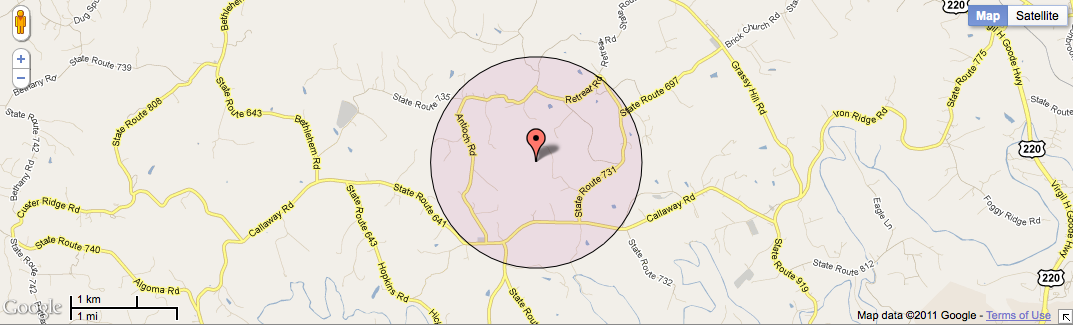
\includegraphics[width=.8\textwidth]{images/google-roadless}
\end{center}
You may need to turn off pop-up blocking for this to work smoothly.
\item
For each map, record whether the center is close (to a road), far (from a road), water, or foreign.
You may need to zoom in or out a bit to figure this out.

\end{enumerate}

\subsection{Variations on the Google Maps theme}

There are many other quantities one could estimate using these tools.  For example:
\begin{enumerate}
\item
What proportion of your home state is within $m$ miles of a lake?  (The choice of $m$ may depend upon
your state of interest.)
\item
Use two proportion procedures  or chi-squared tests to compare states or continents.  
Do all continents have roughly the same proportion of land withing $m$ miles of water (for some $m$)?
Are Utah and Arizona equally roadless?

\item
In more advanced classes: What is the average distance to the nearest lake (in some region)?
By using concentric circles, one could estimate this from discretized data indicating, for example,
whether the nearest lake is within 1/2 mile, between 1/2 mile and 1 mile, between 1 mile and 2 miles,
between 2 miles, and 4 miles, between 4 miles and 10 miles, or more than 10 miles away.  It may be 
interesting to discuss what sort of model should be used for distances from random locations to lakes.
(It probably isn't normally distributed.)
\end{enumerate}

\subsection{Zillow}

\authNote{NH to work with Duncan about expanding the package and its other API}

Zillow.com is an online real estate database that can be used to estimate
property values using tax records, sales data, and comparable homes.  

\centerline{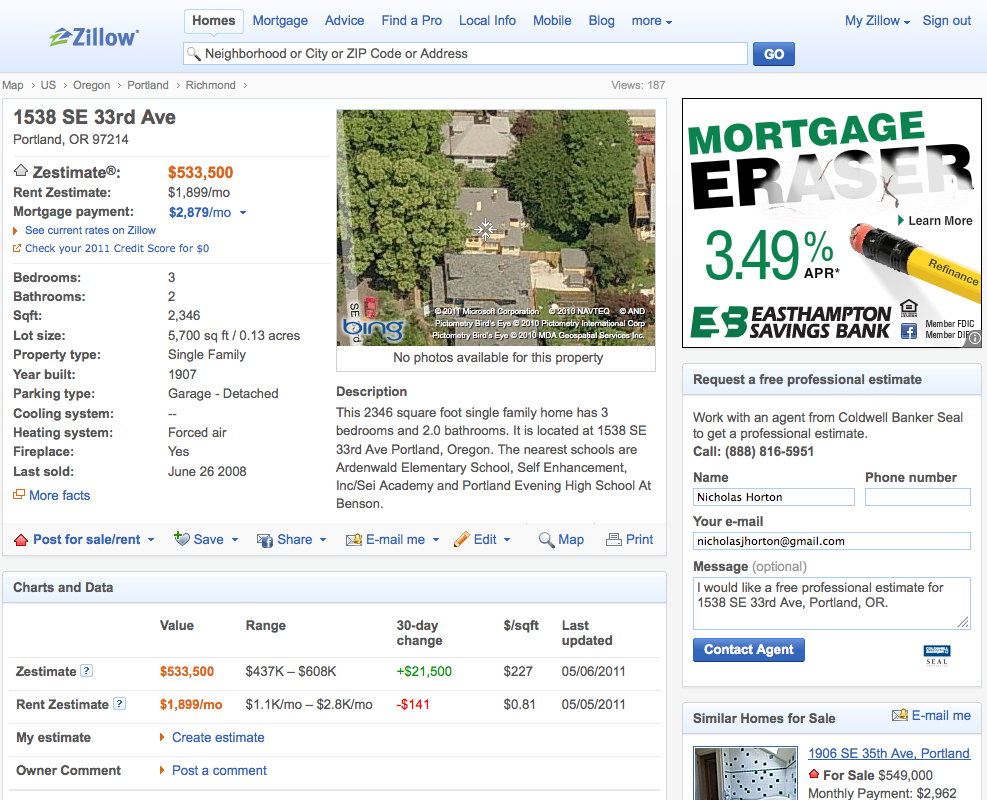
\includegraphics[width=3.8in]{images/zillow1.png}}

The folks who run the site have made an application programming interface (API) 
that specifies 
how software programs can interface with their system.  Duncan Temple Lang has
crafted a package in R that talks to Zillow. 
This can be used to dynamically generate datasets for use in courses, after
you (and/or your students) generate a \VN{zillowId} for use with the system.
(Danny Kaplan has used {\tt cars.com} to similar ends).

\InstructorNote{While this is a cool interface, students tend to be less interested
in house prices than their instructors!}

In this section, we describe how to use Zillow to generate and analyse a
dataset comprised of comparable sites to an arbitrary house of interest.

The first step is to create a Zillow account (click on \verb!Register! on the
top right of the page at \verb!zillow.com!).  You can set up an account or register
using Facebook.
\SuggestionBox{\pkg{Zillow} is new to the authors and we are still looking for 
the ``killer activity'' using \pkg{Zillow}.  We wonder if it is possible, for example,
to sample uniformly among all houses in a city or zip code.}%

Once you have the account, log in, then click on \verb!My Zillow! at the top right.
This should display your profile (in this case, for a user named \verb!SC_z!).

\centerline{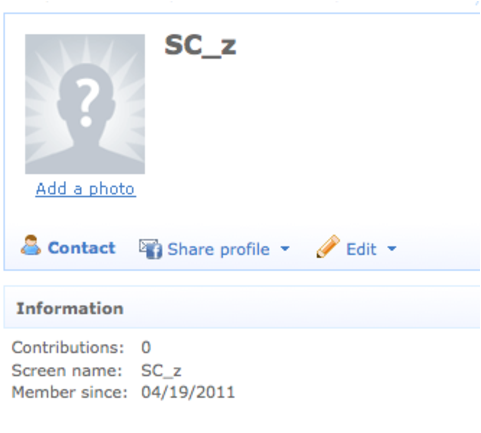
\includegraphics{images/zillow_profile.pdf}}

Next, 
open the page: \url{http://www.zillow.com/webservice/Registration.htm}.  This
is the application programming interface (API) request, which requires more information
if you are a real estate professional.  Note that there are limits on the use 
of these data, which at first glance appear to not contravene use for statistics
activities and data collection. An overview of the API and terms of use can be found
at \url{http://www.zillow.com/howto/api/APIOverview.htm}.

\centerline{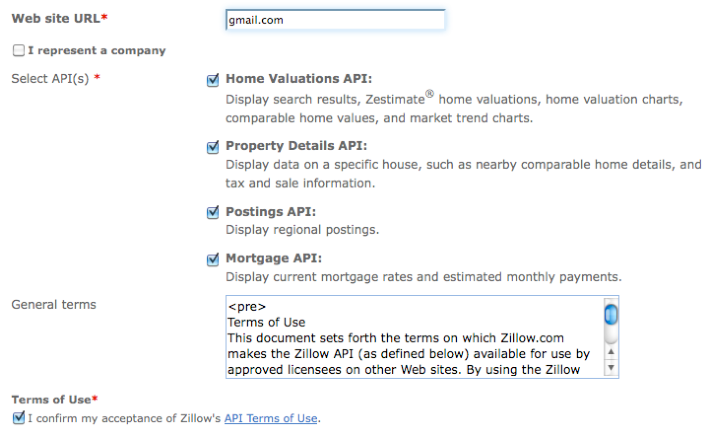
\includegraphics[width=4.6in]{images/zillow_api.pdf}}

You should receive information about your Zillow ID (a character string
of letters and numbers).  

Once you've set up your Zillow account, and gotten your Zillow Id,
the next step is to install the \pkg{Zillow} package. This package is
not on CRAN, but can be obtained from Omegahat (a different repository from CRAN) using
\begin{knitrout}
\definecolor{shadecolor}{rgb}{.97, .97, .97}{\color{fgcolor}\begin{kframe}
\begin{flushleft}
\ttfamily\noindent
\hlfunctioncall{install.packages}\hlkeyword{(}\hlstring{"{}RCurl"{}}\hlkeyword{)}\hspace*{\fill}\\
\hlstd{}\hlfunctioncall{install.packages}\hlkeyword{(}\hlstring{"{}Zillow"{}}\hlkeyword{,}{\ }\hlargument{repos}{\ }\hlargument{=}{\ }\hlstring{"{}http://www.omegahat.org/R"{}}\hlkeyword{,}{\ }\hlargument{type}{\ }\hlargument{=}{\ }\hlstring{"{}source"{}}\hlkeyword{,}\hspace*{\fill}\\
\hlstd{}{\ }{\ }{\ }{\ }\hlargument{dependencies}{\ }\hlargument{=}{\ }\hlstring{"{}Depends"{}}\hlkeyword{)}\mbox{}
\normalfont
\end{flushleft}
\end{kframe}}
\end{knitrout}


Next, you should initialize your \VN{zillowID} to the value that you 
received when you registered with {\tt Zillow.com}.
\begin{knitrout}
\definecolor{shadecolor}{rgb}{.97, .97, .97}{\color{fgcolor}\begin{kframe}
\begin{flushleft}
\ttfamily\noindent
\hlsymbol{zillowId}{\ }\hlassignement{\usebox{\hlnormalsizeboxlessthan}-}{\ }\hlstring{"{}set\usebox{\hlnormalsizeboxunderscore}to\usebox{\hlnormalsizeboxunderscore}your\usebox{\hlnormalsizeboxunderscore}zillowId"{}}\mbox{}
\normalfont
\end{flushleft}
\end{kframe}}
\end{knitrout}




This allows you to make calls to functions such as \function{zestimate()} (which
allows you to search for information about a particular property) and
\function{getComps()} (which facilitates finding a set of comparable properties.  
Here we find information about an arbitrary house in California, as well as
comparable properties.
\begin{knitrout}
\definecolor{shadecolor}{rgb}{.97, .97, .97}{\color{fgcolor}\begin{kframe}
\begin{flushleft}
\ttfamily\noindent
\hlfunctioncall{require}\hlkeyword{(}\hlsymbol{Zillow}\hlkeyword{)}\mbox{}
\normalfont
\end{flushleft}
\begin{verbatim}
Loading required package: Zillow
\end{verbatim}
\begin{verbatim}
Warning message: there is no package called 'Zillow'
\end{verbatim}
\begin{flushleft}
\ttfamily\noindent
\hlsymbol{est}{\ }\hlassignement{\usebox{\hlnormalsizeboxlessthan}-}{\ }\hlfunctioncall{zestimate}\hlkeyword{(}\hlstring{"{}1280{\ }Monterey{\ }Avenue"{}}\hlkeyword{,}{\ }\hlstring{"{}94707"{}}\hlkeyword{,}{\ }\hlsymbol{zillowId}\hlkeyword{)}\mbox{}
\normalfont
\end{flushleft}
\begin{verbatim}
Error: could not find function "zestimate"
\end{verbatim}
\begin{flushleft}
\ttfamily\noindent
\hlsymbol{est}\mbox{}
\normalfont
\end{flushleft}
\begin{verbatim}
Error: object 'est' not found
\end{verbatim}
\begin{flushleft}
\ttfamily\noindent
\hlsymbol{comps}{\ }\hlassignement{\usebox{\hlnormalsizeboxlessthan}-}{\ }\hlfunctioncall{getComps}\hlkeyword{(}\hlfunctioncall{rownames}\hlkeyword{(}\hlsymbol{est}\hlkeyword{)}\hlkeyword{,}{\ }\hlsymbol{zillowId}\hlkeyword{)}\mbox{}
\normalfont
\end{flushleft}
\begin{verbatim}
Error: could not find function "getComps"
\end{verbatim}
\begin{flushleft}
\ttfamily\noindent
\hlfunctioncall{rownames}\hlkeyword{(}\hlsymbol{est}\hlkeyword{)}\mbox{}
\normalfont
\end{flushleft}
\begin{verbatim}
Error: object 'est' not found
\end{verbatim}
\begin{flushleft}
\ttfamily\noindent
\hlfunctioncall{names}\hlkeyword{(}\hlsymbol{comps}\hlkeyword{)}\mbox{}
\normalfont
\end{flushleft}
\begin{verbatim}
Error: object 'comps' not found
\end{verbatim}
\end{kframe}}
\end{knitrout}

\begin{knitrout}
\definecolor{shadecolor}{rgb}{.97, .97, .97}{\color{fgcolor}\begin{kframe}
\begin{flushleft}
\ttfamily\noindent
\hlfunctioncall{table}\hlkeyword{(}\hlsymbol{comps}\hlkeyword{\usebox{\hlnormalsizeboxdollar}}\hlsymbol{bathrooms}\hlkeyword{)}\mbox{}
\normalfont
\end{flushleft}
\begin{verbatim}
Error: object 'comps' not found
\end{verbatim}
\begin{flushleft}
\ttfamily\noindent
\hlfunctioncall{perctable}\hlkeyword{(}\hlsymbol{comps}\hlkeyword{\usebox{\hlnormalsizeboxdollar}}\hlsymbol{bathrooms}\hlkeyword{)}\mbox{}
\normalfont
\end{flushleft}
\begin{verbatim}
Error: object 'comps' not found
\end{verbatim}
\begin{flushleft}
\ttfamily\noindent
\hlfunctioncall{table}\hlkeyword{(}\hlsymbol{comps}\hlkeyword{\usebox{\hlnormalsizeboxdollar}}\hlsymbol{bedrooms}\hlkeyword{)}\mbox{}
\normalfont
\end{flushleft}
\begin{verbatim}
Error: object 'comps' not found
\end{verbatim}
\begin{flushleft}
\ttfamily\noindent
\hlfunctioncall{perctable}\hlkeyword{(}\hlsymbol{comps}\hlkeyword{\usebox{\hlnormalsizeboxdollar}}\hlsymbol{bedrooms}\hlkeyword{)}\mbox{}
\normalfont
\end{flushleft}
\begin{verbatim}
Error: object 'comps' not found
\end{verbatim}
\begin{flushleft}
\ttfamily\noindent
\hlfunctioncall{favstats}\hlkeyword{(}\hlsymbol{comps}\hlkeyword{\usebox{\hlnormalsizeboxdollar}}\hlsymbol{finishedSqFt}\hlkeyword{)}\mbox{}
\normalfont
\end{flushleft}
\begin{verbatim}
Error: object 'comps' not found
\end{verbatim}
\end{kframe}}
\end{knitrout}

We can compare numerical summaries of the size of the house for houses with different 
numbers of bedrooms:
\begin{knitrout}
\definecolor{shadecolor}{rgb}{.97, .97, .97}{\color{fgcolor}\begin{kframe}
\begin{flushleft}
\ttfamily\noindent
\hlfunctioncall{require}\hlkeyword{(}\hlsymbol{Hmisc}\hlkeyword{)}\hspace*{\fill}\\
\hlstd{}\hlfunctioncall{summary}\hlkeyword{(}\hlsymbol{finishedSqFt}{\ }\hlkeyword{\urltilda{}}{\ }\hlsymbol{bedrooms}\hlkeyword{,}{\ }\hlargument{data}{\ }\hlargument{=}{\ }\hlsymbol{comps}\hlkeyword{,}{\ }\hlargument{fun}{\ }\hlargument{=}{\ }\hlsymbol{favstats}\hlkeyword{)}\mbox{}
\normalfont
\end{flushleft}
\begin{verbatim}
Error: object 'comps' not found
\end{verbatim}
\end{kframe}}
\end{knitrout}

We can look at the distribution of Zillow price lower bound, upper bound, as well as assessed
(tax) value.
\InstructorNote{This syntax is somewhat dense, since the \function{bwplot()}
function is expecting a data frame, not 3 vectors}
\begin{knitrout}
\definecolor{shadecolor}{rgb}{.97, .97, .97}{\color{fgcolor}\begin{kframe}
\begin{flushleft}
\ttfamily\noindent
\hlfunctioncall{bwplot}\hlkeyword{(}\hlfunctioncall{rep}\hlkeyword{(}\hlfunctioncall{c}\hlkeyword{(}\hlstring{"{}Low"{}}\hlkeyword{,}{\ }\hlstring{"{}Assessed"{}}\hlkeyword{,}{\ }\hlstring{"{}High"{}}\hlkeyword{)}\hlkeyword{,}{\ }\hlargument{each}{\ }\hlargument{=}{\ }\hlfunctioncall{nrow}\hlkeyword{(}\hlsymbol{comps}\hlkeyword{)}\hlkeyword{)}{\ }\hlkeyword{\urltilda{}}{\ }\hlfunctioncall{c}\hlkeyword{(}\hlsymbol{low}\hlkeyword{,}\hspace*{\fill}\\
\hlstd{}{\ }{\ }{\ }{\ }\hlsymbol{taxAssessment}\hlkeyword{,}{\ }\hlsymbol{high}\hlkeyword{)}\hlkeyword{,}{\ }\hlargument{data}{\ }\hlargument{=}{\ }\hlsymbol{comps}\hlkeyword{,}{\ }\hlargument{horizontal}{\ }\hlargument{=}{\ }\hlnumber{TRUE}\hlkeyword{,}{\ }\hlargument{xlab}{\ }\hlargument{=}{\ }\hlstring{"{}value{\ }(\usebox{\hlnormalsizeboxdollar})"{}}\hlkeyword{)}\mbox{}
\normalfont
\end{flushleft}
\end{kframe}}
\end{knitrout}


As an alternative to the code above, we could first build a data frame and then
use that for our plot.
\InstructorNote{the \pkg{reshape} package also provides support for 
restructuring datasets}
\begin{knitrout}
\definecolor{shadecolor}{rgb}{.97, .97, .97}{\color{fgcolor}\begin{kframe}
\begin{flushleft}
\ttfamily\noindent
\hlsymbol{zillowData}{\ }\hlassignement{\usebox{\hlnormalsizeboxlessthan}-}{\ }\hlfunctioncall{data.frame}\hlkeyword{(}\hlargument{value}{\ }\hlargument{=}{\ }\hlfunctioncall{with}\hlkeyword{(}\hlsymbol{comps}\hlkeyword{,}{\ }\hlfunctioncall{c}\hlkeyword{(}\hlsymbol{low}\hlkeyword{,}{\ }\hlsymbol{taxAssessment}\hlkeyword{,}\hspace*{\fill}\\
\hlstd{}{\ }{\ }{\ }{\ }\hlsymbol{high}\hlkeyword{)}\hlkeyword{)}\hlkeyword{,}{\ }\hlargument{type}{\ }\hlargument{=}{\ }\hlfunctioncall{rep}\hlkeyword{(}\hlfunctioncall{c}\hlkeyword{(}\hlstring{"{}Low"{}}\hlkeyword{,}{\ }\hlstring{"{}Assessed"{}}\hlkeyword{,}{\ }\hlstring{"{}High"{}}\hlkeyword{)}\hlkeyword{,}{\ }\hlargument{each}{\ }\hlargument{=}{\ }\hlfunctioncall{nrow}\hlkeyword{(}\hlsymbol{comps}\hlkeyword{)}\hlkeyword{)}\hlkeyword{)}\hspace*{\fill}\\
\hlstd{}\hlfunctioncall{bwplot}\hlkeyword{(}\hlsymbol{value}{\ }\hlkeyword{\urltilda{}}{\ }\hlsymbol{type}\hlkeyword{,}{\ }\hlsymbol{zillowData}\hlkeyword{)}\mbox{}
\normalfont
\end{flushleft}
\end{kframe}}
\end{knitrout}


It's interesting that for these properties, assessed values tend to be lower
that both the lower and upper Zillow estimates.  
We could explore whether this is true in California more generally.

It's possible to plot the results of our comparable properties, which yields a scatterplot
of price by square feet (with the number of bedrooms as well as the low and high range) as
well as a scatterplot of amount/finished square feet vs log size in square feet.
\begin{knitrout}
\definecolor{shadecolor}{rgb}{.97, .97, .97}{\color{fgcolor}\begin{kframe}
\begin{flushleft}
\ttfamily\noindent
\hlfunctioncall{plot}\hlkeyword{(}\hlsymbol{comps}\hlkeyword{)}\mbox{}
\normalfont
\end{flushleft}
\end{kframe}}
\end{knitrout}


Several aspects of this activity are worth noting: 
\begin{enumerate}
\item There is some startup cost for instructors and students (since each user will need
their own ZillowID\footnote{By default, the number of calls per day to the API is limited to 1000,
which could easily be exceeded in a lab setting if, contrary to the terms of use, the Zillow ID
were to be shared.}).  
\item Once set up, the calls to the Zillow package are very straightforward, and provide
immediate access to a wealth of interesting data.
\item This could be used as an activity to provide descriptive analysis of comparable 
properties, or in a more elaborate manner to compare properties in different cities or
areas.
\item Since the latitude and longitude of the comparable properties is returned, users
can generate maps using the mechanisms described in \ref{sec:googleMap}.
\end{enumerate}

\subsection{Twitter}
\label{sec:twitter}

\authNote{NH to reimplement the proposed interface}

Twitter (\url{twitter.com}) is a social networking and microblogging service, where users
(estimated at 200 million as of May, 2011) can send and read posts of up to 140 characters.
Approximately 65 million ``tweets'' are posted per day.

The \pkg{twitteR} package (due to Jeff Gentry) implements a Twitter client for R.
This can be used to generate data for student projects, class assignments or data mining.

\Caution{Pulling live data from Twitter may generate some unsavory content}

The package provides a number of interface functions to connect with the service (see
Table \ref{tab:twitter} for details).
\begin{table}
\begin{center}
\caption{Functions available within the \pkg{twitteR} package}
\label{tab:twitter}
\begin{tabular}{|l|l|l|} \hline
Function   & Description                 \\ \hline
\function{getUser} & returns an object of class {\tt user} \\
\function{userFriends} & returns lists of class {\tt user} \\
\function{userFollowers} & returns a list of class {\tt user} \\
\function{searchTwitter} & returns a list of class {\tt status} \\
\function{Rtweets} & search for {\tt \#rstats} \\
\function{showstatus} & take a numeric ID of a tweet and return it \\
\function{publicTimeline} & current snapshot of the public timeline \\
\function{userTimeline} & current snapshot of the users public timeline \\ \hline
\end{tabular}
\end{center}
\end{table}


Some examples may help to better understand the interface.  Let's start by seeing what 
the U.S. Census Bureau has been up to recently.
\begin{knitrout}
\definecolor{shadecolor}{rgb}{.97, .97, .97}{\color{fgcolor}\begin{kframe}
\begin{flushleft}
\ttfamily\noindent
\hlfunctioncall{require}\hlkeyword{(}\hlsymbol{twitteR}\hlkeyword{)}\mbox{}
\normalfont
\end{flushleft}
\begin{verbatim}
Loading required package: twitteR
\end{verbatim}
\begin{verbatim}
Warning message: there is no package called 'twitteR'
\end{verbatim}
\begin{flushleft}
\ttfamily\noindent
\hlsymbol{census}{\ }\hlassignement{\usebox{\hlnormalsizeboxlessthan}-}{\ }\hlfunctioncall{getUser}\hlkeyword{(}\hlstring{"{}uscensusbureau"{}}\hlkeyword{)}\mbox{}
\normalfont
\end{flushleft}
\begin{verbatim}
Error: could not find function "getUser"
\end{verbatim}
\begin{flushleft}
\ttfamily\noindent
\hlsymbol{census}\hlkeyword{\usebox{\hlnormalsizeboxdollar}}\hlfunctioncall{getName}\hlkeyword{(}\hlkeyword{)}\mbox{}
\normalfont
\end{flushleft}
\begin{verbatim}
Error: object 'census' not found
\end{verbatim}
\begin{flushleft}
\ttfamily\noindent
\hlsymbol{census}\hlkeyword{\usebox{\hlnormalsizeboxdollar}}\hlfunctioncall{getDescription}\hlkeyword{(}\hlkeyword{)}\mbox{}
\normalfont
\end{flushleft}
\begin{verbatim}
Error: object 'census' not found
\end{verbatim}
\begin{flushleft}
\ttfamily\noindent
\hlsymbol{census}\hlkeyword{\usebox{\hlnormalsizeboxdollar}}\hlfunctioncall{getUrl}\hlkeyword{(}\hlkeyword{)}\mbox{}
\normalfont
\end{flushleft}
\begin{verbatim}
Error: object 'census' not found
\end{verbatim}
\begin{flushleft}
\ttfamily\noindent
\hlsymbol{census}\hlkeyword{\usebox{\hlnormalsizeboxdollar}}\hlfunctioncall{getStatusesCount}\hlkeyword{(}\hlkeyword{)}\mbox{}
\normalfont
\end{flushleft}
\begin{verbatim}
Error: object 'census' not found
\end{verbatim}
\begin{flushleft}
\ttfamily\noindent
\hlsymbol{census}\hlkeyword{\usebox{\hlnormalsizeboxdollar}}\hlfunctioncall{getCreated}\hlkeyword{(}\hlkeyword{)}\mbox{}
\normalfont
\end{flushleft}
\begin{verbatim}
Error: object 'census' not found
\end{verbatim}
\begin{flushleft}
\ttfamily\noindent
\hlsymbol{census}\hlkeyword{\usebox{\hlnormalsizeboxdollar}}\hlfunctioncall{getFollowersCount}\hlkeyword{(}\hlkeyword{)}\mbox{}
\normalfont
\end{flushleft}
\begin{verbatim}
Error: object 'census' not found
\end{verbatim}
\end{kframe}}
\end{knitrout}

That's a lot of followers (but then again, the census is a big job).  
Detailed reports of the last set of twitter status updates can be returned.
Let's take a look at what William Shatner has been up to.
\begin{knitrout}
\definecolor{shadecolor}{rgb}{.97, .97, .97}{\color{fgcolor}\begin{kframe}
\begin{flushleft}
\ttfamily\noindent
\hlsymbol{shatner.tweets}{\ }\hlassignement{\usebox{\hlnormalsizeboxlessthan}-}{\ }\hlfunctioncall{userTimeline}\hlkeyword{(}\hlstring{"{}williamshatner"{}}\hlkeyword{,}{\ }\hlargument{n}{\ }\hlargument{=}{\ }\hlnumber{5}\hlkeyword{)}\mbox{}
\normalfont
\end{flushleft}
\begin{verbatim}
Error: could not find function "userTimeline"
\end{verbatim}
\end{kframe}}
\end{knitrout}

By default, the tweets don't print very nicely.  So let's define our 
own function to extract the text from a tweet and format it more
nicely.
\begin{knitrout}
\definecolor{shadecolor}{rgb}{.97, .97, .97}{\color{fgcolor}\begin{kframe}
\begin{flushleft}
\ttfamily\noindent
\hlsymbol{printTweet}{\ }\hlassignement{\usebox{\hlnormalsizeboxlessthan}-}{\ }\hlkeyword{function}\hlkeyword{(}\hlformalargs{x}\hlkeyword{)}{\ }\hlfunctioncall{paste}\hlkeyword{(}\hlfunctioncall{strwrap}\hlkeyword{(}\hlsymbol{x}\hlkeyword{\usebox{\hlnormalsizeboxdollar}}\hlfunctioncall{getText}\hlkeyword{(}\hlkeyword{)}\hlkeyword{)}\hlkeyword{)}\hspace*{\fill}\\
\hlstd{}\hlfunctioncall{printTweet}\hlkeyword{(}\hlsymbol{shatner.tweets}\hlkeyword{[[}\hlnumber{1}\hlkeyword{]}\hlkeyword{]}\hlkeyword{)}\mbox{}
\normalfont
\end{flushleft}
\begin{verbatim}
Error: object 'shatner.tweets' not found
\end{verbatim}
\end{kframe}}
\end{knitrout}

Detailed information can be found for individual tweets.

\begin{knitrout}
\definecolor{shadecolor}{rgb}{.97, .97, .97}{\color{fgcolor}\begin{kframe}
\begin{flushleft}
\ttfamily\noindent
\hlsymbol{shatner.tweets}\hlkeyword{[[}\hlnumber{1}\hlkeyword{]}\hlkeyword{]}\hlkeyword{\usebox{\hlnormalsizeboxdollar}}\hlfunctioncall{getCreated}\hlkeyword{(}\hlkeyword{)}\mbox{}
\normalfont
\end{flushleft}
\begin{verbatim}
Error: object 'shatner.tweets' not found
\end{verbatim}
\begin{flushleft}
\ttfamily\noindent
\hlsymbol{shatner.tweets}\hlkeyword{[[}\hlnumber{1}\hlkeyword{]}\hlkeyword{]}\hlkeyword{\usebox{\hlnormalsizeboxdollar}}\hlfunctioncall{getId}\hlkeyword{(}\hlkeyword{)}\mbox{}
\normalfont
\end{flushleft}
\begin{verbatim}
Error: object 'shatner.tweets' not found
\end{verbatim}
\end{kframe}}
\end{knitrout}

\DiggingDeeper{Section \ref{sec:datastruct} provides details on accessing lists.}

Using \function{sapply()}, we can inspect all of the tweets at once.
\begin{knitrout}
\definecolor{shadecolor}{rgb}{.97, .97, .97}{\color{fgcolor}\begin{kframe}
\begin{flushleft}
\ttfamily\noindent
\hlfunctioncall{sapply}\hlkeyword{(}\hlsymbol{shatner.tweets}\hlkeyword{,}{\ }\hlsymbol{printTweet}\hlkeyword{)}\mbox{}
\normalfont
\end{flushleft}
\begin{verbatim}
Error: object 'shatner.tweets' not found
\end{verbatim}
\end{kframe}}
\end{knitrout}

\DiggingDeeper{the \function{sapply()} applies a function to each element of a list
or vector.  It is one of several ``apply'' functions in \R, including
\function{apply}, and 
\function{sapply}, and 
\function{lapply}, and 
\function{tapply}.
The \pkg{mosaic} package even include
\function{dfapply} for application to data frames.}

Alternatively, we can download information about how active Census Bureau followers are 
in terms of posting their own status updates.

\begin{knitrout}
\definecolor{shadecolor}{rgb}{.97, .97, .97}{\color{fgcolor}\begin{kframe}
\begin{flushleft}
\ttfamily\noindent
\hlsymbol{userFollowers}{\ }\hlassignement{=}{\ }\hlkeyword{function}\hlkeyword{(}\hlformalargs{user}\hlkeyword{)}{\ }\hlkeyword{\usebox{\hlnormalsizeboxopenbrace}}\hspace*{\fill}\\
\hlstd{}{\ }{\ }{\ }{\ }\hlfunctioncall{return}\hlkeyword{(}\hlsymbol{user}\hlkeyword{\usebox{\hlnormalsizeboxdollar}}\hlfunctioncall{getUserFollowers}\hlkeyword{(}\hlkeyword{)}\hlkeyword{)}\hspace*{\fill}\\
\hlstd{}\hlkeyword{\usebox{\hlnormalsizeboxclosebrace}}\hspace*{\fill}\\
\hlstd{}\hlsymbol{census.followers}{\ }\hlassignement{\usebox{\hlnormalsizeboxlessthan}-}{\ }\hlfunctioncall{userFollowers}\hlkeyword{(}\hlsymbol{census}\hlkeyword{)}\hspace*{\fill}\\
\hlstd{}\hlsymbol{followers.ntweets}{\ }\hlassignement{\usebox{\hlnormalsizeboxlessthan}-}{\ }\hlfunctioncall{sapply}\hlkeyword{(}\hlsymbol{census.followers}\hlkeyword{,}{\ }\hlkeyword{function}\hlkeyword{(}\hlformalargs{x}\hlkeyword{)}{\ }\hlsymbol{x}\hlkeyword{\usebox{\hlnormalsizeboxdollar}}\hlfunctioncall{getStatusesCount}\hlkeyword{(}\hlkeyword{)}\hlkeyword{)}\hspace*{\fill}\\
\hlstd{}\hlfunctioncall{favstats}\hlkeyword{(}\hlsymbol{followers.ntweets}\hlkeyword{)}\hspace*{\fill}\\
\hlstd{}\hlsymbol{census.followers}\hlkeyword{[[}\hlfunctioncall{which.max}\hlkeyword{(}\hlsymbol{followers.ntweets}\hlkeyword{)}\hlkeyword{]}\hlkeyword{]}\mbox{}
\normalfont
\end{flushleft}
\end{kframe}}
\end{knitrout}

That's probably a bit much for students to swallow.  Let's write a function to hide 
some of the gory details from the students.
\begin{knitrout}
\definecolor{shadecolor}{rgb}{.97, .97, .97}{\color{fgcolor}\begin{kframe}
\begin{flushleft}
\ttfamily\noindent
\hlsymbol{CountTweets}{\ }\hlassignement{\usebox{\hlnormalsizeboxlessthan}-}{\ }\hlkeyword{function}\hlkeyword{(}\hlformalargs{users}\hlkeyword{)}{\ }\hlkeyword{\usebox{\hlnormalsizeboxopenbrace}}\hspace*{\fill}\\
\hlstd{}{\ }{\ }{\ }{\ }\hlfunctioncall{return}\hlkeyword{(}\hlfunctioncall{sapply}\hlkeyword{(}\hlsymbol{users}\hlkeyword{,}{\ }\hlkeyword{function}\hlkeyword{(}\hlformalargs{x}\hlkeyword{)}{\ }\hlsymbol{x}\hlkeyword{\usebox{\hlnormalsizeboxdollar}}\hlfunctioncall{getStatusesCount}\hlkeyword{(}\hlkeyword{)}\hlkeyword{)}\hlkeyword{)}\hspace*{\fill}\\
\hlstd{}\hlkeyword{\usebox{\hlnormalsizeboxclosebrace}}\mbox{}
\normalfont
\end{flushleft}
\end{kframe}}
\end{knitrout}

Now we can count tweets like this.
\begin{knitrout}
\definecolor{shadecolor}{rgb}{.97, .97, .97}{\color{fgcolor}\begin{kframe}
\begin{flushleft}
\ttfamily\noindent
\hlfunctioncall{sort}\hlkeyword{(}\hlfunctioncall{CountTweets}\hlkeyword{(}\hlsymbol{census.followers}\hlkeyword{)}\hlkeyword{)}\mbox{}
\normalfont
\end{flushleft}
\end{kframe}}
\end{knitrout}



We can also see what's happening on the \R\ front:
\begin{knitrout}
\definecolor{shadecolor}{rgb}{.97, .97, .97}{\color{fgcolor}\begin{kframe}
\begin{flushleft}
\ttfamily\noindent
\hlsymbol{R.tweets}{\ }\hlassignement{\usebox{\hlnormalsizeboxlessthan}-}{\ }\hlfunctioncall{Rtweets}\hlkeyword{(}\hlargument{n}{\ }\hlargument{=}{\ }\hlnumber{5}\hlkeyword{)}{\ }{\ }\hlcomment{\usebox{\hlnormalsizeboxhash}{\ }short{\ }for{\ }searchTwitter(\usebox{\hlnormalsizeboxsinglequote}\usebox{\hlnormalsizeboxhash}rstats\usebox{\hlnormalsizeboxsinglequote},{\ }n=5)}\mbox{}
\normalfont
\end{flushleft}
\begin{verbatim}
Error: could not find function "Rtweets"
\end{verbatim}
\begin{flushleft}
\ttfamily\noindent
\hlfunctioncall{sapply}\hlkeyword{(}\hlsymbol{R.tweets}\hlkeyword{,}{\ }\hlsymbol{printTweet}\hlkeyword{)}\mbox{}
\normalfont
\end{flushleft}
\begin{verbatim}
Error: object 'R.tweets' not found
\end{verbatim}
\end{kframe}}
\end{knitrout}


\authNote{DTK: I get no hits on this search as of May 29.  Perhaps
  tags time out or \texttt{searchTwitter} only looks at recent activity.}

Finally, we can see who has been tweeting the most at USCOTS:
\begin{knitrout}
\definecolor{shadecolor}{rgb}{.97, .97, .97}{\color{fgcolor}\begin{kframe}
\begin{flushleft}
\ttfamily\noindent
\hlfunctioncall{sort}\hlkeyword{(}\hlfunctioncall{table}\hlkeyword{(}\hlfunctioncall{sapply}\hlkeyword{(}\hlfunctioncall{searchTwitter}\hlkeyword{(}\hlstring{"{}\usebox{\hlnormalsizeboxhash}uscots11"{}}\hlkeyword{)}\hlkeyword{,}{\ }\hlkeyword{function}\hlkeyword{(}\hlformalargs{x}\hlkeyword{)}{\ }\hlsymbol{x}\hlkeyword{\usebox{\hlnormalsizeboxdollar}}\hlfunctioncall{getScreenName}\hlkeyword{(}\hlkeyword{)}\hlkeyword{)}\hlkeyword{)}\hlkeyword{,}\hspace*{\fill}\\
\hlstd{}{\ }{\ }{\ }{\ }\hlargument{decreasing}{\ }\hlargument{=}{\ }\hlnumber{TRUE}\hlkeyword{)}\mbox{}
\normalfont
\end{flushleft}
\end{kframe}}
\end{knitrout}

\InstructorNote{Support functions could be written to simplify this interface for 
student use.  Just another thing for us to do in our spare time...}

\author

Further support for posting tweets requires use of the Twitter API (with appropriate 
authentication).  More details are provided in the \pkg{twitteR} vignette file.

\subsection{Other ideas}

We've outlined several approaches which efficiently scrape data from the web.
But there are lots of other examples which may be worth exploring (and this is clearly 
a growth area).  These include:
\begin{description}
\item[\pkg{RNYTimes}] interface to several of the \emph{New York Times} web services
for searching articles, meta-data, user-generated content and best seller lists 
(\url{http://www.omegahat.org/RNYTimes})
\item[\pkg{Rflickr}] interface to the Flickr photo sharing service 
(\url{http://www.omegahat.org/Rflickr})
\item[\pkg{RGoogleDocs}] interface to allow listing documents on Google Docs 
along with details, downloading contents, and uploading files 
(\url{http://www.omegahat.org/RGoogleDocs})
\item[\pkg{RLastFM}] interface to the \verb!last.fm! music recommendation site (\url{http://cran.r-project.org/web/packages/RLastFM})
\end{description}

